\documentclass[a4paper,12pt]{report}
\usepackage[utf8]{inputenc}
\usepackage{enumitem}
\usepackage[colorinlistoftodos]{todonotes}
\usepackage{hyperref}

\begin{document}

\chapter{Protocolo HTTP}

\section{Descripción}
HTTP es un protocolo de capa de aplicación, genérico, sin estado, del tipo cliente-servidor, utilizado en sistemas de información distribuidos y colaborativos.
Desarrollado por la Internet Engineering Task Force (IETF) y la World Wide Web Consortium (W3C), culminando en la publicación de una serie de \emph{rfcs},
siendo el rfc 2616 \cite{rfc2616} el más notorio, en el cual se encuentra especificada la versión HTTP 1.1.

\section{Compresión}

El tamaño de la respuesta HTTP puede ser reducido comprimiendo su contenido, si tanto el servidor como el navegador pueden procesar elementos comprimidos.
Los navegadores comunican al servidor que tipo de compresión soportan mediante el uso del encabezado \texttt{Accept-Encoding} definido en el rfc 2616 \cite{rfc2616} sección 14.3.
Por otro lado los servidores identifican una respuesta comprimida mediante el uso del encabezado \texttt{Content-Encoding} definido en el rfc 2616 \cite{rfc2616} sección 14.11.

\begin{figure}[h]
\centering
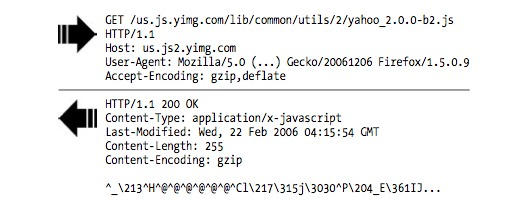
\includegraphics[width=1\textwidth]{figuras/apendice/compression.jpg}
  \caption{Ejemplo de pedido y respuesta HTTP con compresión.}
    \label{fig.compresion}
\end{figure}

Como se puede ver en la figura \ref{fig.compresion} el pedido HTTP contiene el encabezado \texttt{Accept-Encoding}, indicándole al servidor que acepta elementos comprimidos
con el formato gzip y deflate. La respuesta del servidor contiene el encabezado \texttt{Content-Encoding} indicando el formato en el cual se encuentra comprimido
el cuerpo de la respuesta.

\section{Pedidos condicionales}

Se realiza un pedido condicional cuando el navegador tiene una copia del elemento que se quiere obtener en su cache. En este caso, el navegador debe verificar con el servidor
si la copia que tiene almacenada en su \emph{cache} sigue siendo válida.
La validez de la copia es determinada en base a la fecha en la que el elemento fue modificado por última vez. La presencia del encabezado \texttt{Last-Modified}
especificado en el rfc 2616 \cite{rfc2616} sección 14.29 en la respuesta HTTP, permite a los navegadores saber cuándo fue la última vez que un elemento fue modificado.

\begin{figure}[h]
\centering
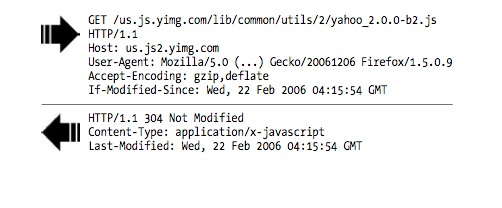
\includegraphics[width=1\textwidth]{figuras/apendice/condicional.jpg}
	\caption{Ejemplo de pedido y respuesta HTTP condicionales.}
    \label{fig.condicional}
\end{figure}

El navegador realiza un pedido condicional enviando el encabezado \texttt{If-Modified-Since} (especificado en el rfc 2616 \cite{rfc2616} sección 14.25) con la fecha que tiene el elemento
en su cache como se puede apreciar en \ref{fig.condicional}, consultando al servidor si el elemento fue modificado desde la fecha.
En caso en que no haya sido modificado, el servidor envía una respuesta \texttt{304 Not-Modified} sin cuerpo, en otro caso el servidor envía la nueva versión del elemento
en el cuerpo de la respuesta, haciendo que la misma sea de mayor tamaño.

\subsection{If-Match}
El encabezado \emph{If-match} es utilizado para hacer que un método sea condicional. Un cliente que tiene una o más entidades que previamente obtenidas de un recurso puede
verificar que una de esas entidades es actual al incluir una lista de las \emph{entity tags} asociadas a ellas en el encabezado \emph{If-Match}. Es utilizado para realizar
actualizaciones de información almacenada en caches de manera efectiva con un mínimo overhead de transacción.

Un servidor debe utilizar la función de comparación fuerte para comparar \emph{entity tags} en presencia del encabezado \emph{If-Match}. Si ninguna de las \emph{entity tags}
iguala, o si el valor del encabezado es\emph{*} y no existen entidades, el servidor debe ejecutar el método de la respuesta y debe retornar una respuesta con estado 412. Este
comportamiento es útil cuando un cliente quiere prevenir que un método de actualización como el PUT modifique un recurso que ha cambiado desde que el cliente lo obtuvo por última
vez.

Si el pedido resultara en una respuesta con un código distinto de 2xx o 412 (en caso de no contener el encabezado \emph{If-Match}), entonces el encabezado \emph{If-Match} debe
ser ignorado.

\subsection{If-Modified-Since}
Este encabezado es utilizado para realizar un pedido condicional: si la entidad solicitada no ha sido modificada desde el tiempo especificado en este encabezado, la
misma no será retornada por el servidor, en su lugar, ser retornara una respuesta con estado 304 y sin cuerpo.

Un pedido \emph{GET} con este encabezado que no contenga el encabezado \emph{Range}, pide que la entidad identificada sea transferida solo si ha sido modificada desde la fecha
presente en este encabezado. El algoritmo consiste de tres pasos. En primer lugar, si la respuesta normalmente resultaría en un código distinto de 200 o si la fecha presente
en el encabezado \emph{If-Modified-Since} es invalida, la respuesta debe ser la misma que en un pedido \emph{GET} tradicional. Una fecha es inválida si es mayor que la fecha
actual del servidor. En caso que la entidad haya sido modificada desde la fecha incluida en este cabezal, la respuesta debe ser la misma que para un \emph{GET} condicional.
Si la entidad no ha sido modificada desde una fecha valida \emph{If-modified-Since}, el servidor debe retornar una respuesta con código 304.

\subsection{If-None-Match}
Es utilizado para realizar pedidos condicionales.  Un cliente que tiene una o más entidades que previamente obtenidas de un recurso puede
verificar que ninguna de esas entidades es actual al incluir una lista de las \emph{entity tags} asociadas a ellas en el encabezado \emph{If-None-Match}. Es utilizado para realizar
actualizaciones de información almacenada en caches de manera efectiva con un mínimo overhead de transacción. También es utilizado para prevenir que métodos como \emph{PUT}
modifiquen de forma inadvertida un recurso existente cuando un cliente cree que ese recurso no existe.

Si alguna de las \emph{entity tags} coincide con la \emph{entity tag} de la entidad que hubiera sido retornada en respuesta a un pedido \emph{GET} similar (sin el encabezado
\emph{If-None-Match}), o si \emph{*} es el valor de este encabezado y existe una entidad actual de ese recurso, entonces el servidor no debe ejecutar el método del pedido.
El caso particular en el cual el servidor debe ejecutar el método se da cuando la fecha de modificación del recurso no coincide con la provista en el encabezado
\emph{If-Modified-Since}.

En cambio si el método del pedido es \emph{GET} o \emph{HEAD}, el servidor debe responder con un estado 304, incluyendo los encabezado relacionados con el cache de una de las
entidades que coincidió. Para todos los demás métodos, el servidor debe responder con un estado 422.
Instead, if the request method was GET or HEAD, the server SHOULD

Si ninguna de las \emph{entity tags} coincidieron, el servidor puede ejecutar el método del pedido como si el encabezado \emph{If-None-Match} no fuera parte del pedido, pero
también debe ignorar cualquier encabezado \emph{If-Modified-Since} presentes en el pedido. Esto quiere decir que si ninguna \emph{entity tag} coincide, el servidor no debe
retornar una respuesta con estado 304.

\section{Expires}

Pedidos condicionales y respuestas del tipo 304 permiten que los sitios se carguen más rápido, pero sigue requiriendo un intercambio de mensajes entre el cliente y el servidor
para realizar la validación. El encabezado \texttt{Expires} (especificado en el rfc 2616 \cite{rfc2616} sección 14.21) elimina la necesidad de validar con
servidor, indicando al navegador hasta cuándo puede utilizar el elemento que se encuentra en el cuerpo de la respuesta.

\begin{figure}[h]
\centering
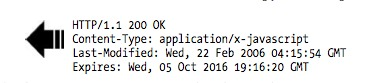
\includegraphics[width=1\textwidth]{figuras/apendice/expires.jpg}
	\caption{Ejemplo de respuesta con el encabezado \texttt{Expires}.}
    \label{fig.expires}
\end{figure}

Cuando un navegador recibe una respuesta con el encabezado \texttt{Expires}, almacena la fecha de expiración indicada en el encabezado, junto con el componente en su cache.
Mientras que el componente no haya expirado el navegador continuará usando la versión del elemento que tiene en su cache, evitando de esta forma realizar pedidos HTTP.

\section{Keep-Alive}

HTTP utiliza como protocolo de capa de transporte a TCP especificado en el rfc 793 \cite{rfc793}. En implementaciones anteriores, cada pedido HTTP requería
iniciar una conexión nueva a través de un socket. Esto es ineficiente ya que la mayoría de los pedidos en un sitio se realizan al mismo servidor.
Las conexiones persistentes (\texttt{Keep-Alive en HTTP/1.0}) fueron introducidas para resolver la ineficiencia de iniciar y cerrar conexiones al mismo servidor, permitiendo
a los navegadores realizar múltiples pedidos HTTP de manera secuencial mediante una sola conexión.

El soporte de conexiones persistentes por parte de los navegadores y servidores es indicado mediante la inclusión del encabezado \texttt{Connection}
especificado en el rfc 2616 \cite{rfc2616} sección 14.10.

\begin{figure}[h]
\centering
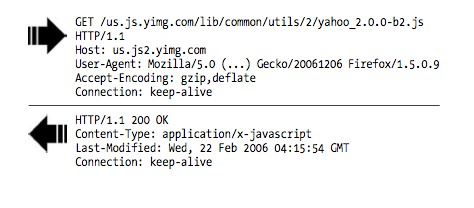
\includegraphics[width=1\textwidth]{figuras/apendice/keep-alive.jpg}
	\caption{Ejemplo de pedido y respuesta con el encabezado \texttt{Connection}.}
    \label{fig.keep-alive}
\end{figure}

Tanto el navegador como el servidor pueden cerrar la conexión, incluyendo en el paquete HTTP el encabezado \texttt{Connection: close}.

\section{Warnings}

El encabezado \emph{Warning} es utilizado para enviar información adicional sobre el estado o la transformación de un mensaje que puede no ser reflejada en el mismo.
Esta información es típicamente utilizada para advertir sobre la posible falta de transparencia semántica producto de operaciones o transformaciones de cache
aplicadas al cuerpo de la entidad del mensaje.

Un cache es semánticamente transparente respecto a una respuesta particular, cuando su uso no afecta al cliente ni al servidor, solo mejora la performance. El cliente
recibe exactamente la misma respuesta  que hubiera recibido si su pedido hubiera sido atendido por el servidor de origen.
El encabezado \emph{Warning} es incluido en las respuestas y tiene el siguiente formato:


       Warning    = 'Warning' ':' 1\#warning-value

       warning-value = warn-code SP warn-agent SP warn-text
                                             [SP warn-date]

       warn-code  = 3DIGIT

       warn-agent = ( host [ ':' port ] ) | pseudonym
                       ; the name or pseudonym of the server adding
                       ; the Warning header, for use in debugging

       warn-text  = quoted-string

       warn-date  = 'HTTP-date'


El campo \emph{warn-text} debe estar en lenguaje natural y el conjunto de caracteres utilizado debe poder ser comprendido por el individuo que recibe la respuesta. Esta
información puede ser basada en el valor del encabezado \emph{Accept-Language} del pedido, el valor del encabezado \emph{Content-Language} de la respuesta o de la ubicación
del usuario entre otros. El lenguaje por defecto según la especificación es Ingles y el conjunto de caracteres es ISO-8859-1.

Los encabezados \emph{Warning} en general pueden ser aplicados a cualquier mensaje, pero algunos \emph{warn-codes} son específicos para caches y pueden ser aplicados solo
a respuestas. Encabezados del tipo \emph{Warning} deben ser agregados en caso de que ya exista alguno en la respuesta, un cache no puede eliminar ningún encabezado
de este tipo que se encuentre en una respuesta que recibe.

Cuando una respuesta contiene varios encabezados \emph{Warning}, el \emph{user-agent} debe informar al usuario de todas las que pueda en el orden en que aparecen en la
respuesta. En caso de no poder informar de todas, el \emph{user-agent} debe aplicar una de las siguientes heurísticas. Las que aparecen antes en la respuesta tienen prioridad
sobre las que aparecen después, y las que aparecen en el conjunto de caracteres preferido del usuario tienen mayor prioridad sobre las que tienen otro conjunto de caracteres
pero idénticos \emph{warn-codes} y \emph{warn-agents}.

\section{Cache-Control}
Este encabezado es utilizado para especificar directivas que deben ser obedecidas por todos los mecanismos de cache a lo largo de la cadena de pedido/respuesta.
Estas directivas especifican comportamiento destinado a prevenir que los caches interfieran de forma adversa los pedidos y las respuestas. Las mismas sobrescriben los
algoritmos por defecto de cache.

Cuando una directiva aparece sin el parámetro \emph{1\#field-name}, la misma aplica a todo el pedido o respuesta, en cambio cuando la misma está presente con este parámetro
aplica solo al o los campos \emph{1\#field-name} y no a la totalidad del pedio o respuesta.
Las directivas de \emph{Cache-Control} se pueden clasificar de la siguiente manera:

\begin{enumerate}
  \item Restricciones de lo que puede guardarse en \emph{cache}, estas solo pueden ser impuestas por el servidor de origen.
  \item Restricciones sobre lo que puede ser almacenado en cache, pueden ser impuestas tanto por el servidor de origen como por el \emph{user-agent}.
  \item Modificaciones a los mecanismos básicos de expiración, pueden ser impuestas por el servidor de origen o el \emph{user-agent}.
  \item Controles sobre la revalidación de cache, pueden ser impuestos solo por el \emph{user-agent}
  \item controles sobre la transformación de entidades.
  \item Extensiones al sistema de cache.
\end{enumerate}

\subsection{Directivas de Cache-Control}
Por defecto una respuesta puede almacenarse en un cache si los requerimientos del método del pedido, los campos de los encabezados y el código de estado de la misma lo
indican. Las siguientes directivas de \emph{Cache-Control} permiten al servidor de origen sobrescribir la \emph{cacheabilidad} de una respuesta

\begin{enumerate}
  \item \textbf{public} Indica que la la respuesta puede ser almacenada en cache por cualquier cache, aun cuando normalmente no lo seria.
  \item \textbf{private} Indica que todo o parte del mensaje de la respuesta puede ser almacenada en cache por un cache distribuido. Esto
  permite al servidor de origen especificar que determinadas parte de la respuesta son destinadas únicamente para un usuario y no son válidas para pedidos de otros usuarios.
  \item \textbf{no-cache} Si esta directiva no especifica un \emph{field-name} entonces un cache no debe utilizar la respuestas para satisfacer subsiguientes pedidos sin
  revalidar de manera exitosa con el servidor de origen. En cambio si la directiva incluye uno o varios \emph{field-names}, un cache puede utilizar la respuesta para
  satisfacer subsiguientes pedidos, teniendo en cuenta cualquier otra restricción de cache. Sin embargo los \emph{field-names} especificados no deben ser enviados en subsiguientes
  respuestas sin una revalidación exitosa del servidor de origen. Esto permite al servidor de origen prevenir la reutilización de ciertos campos de algunos encabezados, mientras
  que sigue permitiendo que el resto de la respuesta pueda ser almacenada en cache.
  \item \textbf{no-store} El propósito de esta directiva es prevenir la emisión inadvertida o retención de información sensible. Esta directiva aplica al mensaje en su
  totalidad y puede ser enviada en una respuesta o en un pedido. En caso de ser enviada en un pedido un cache no debe almacenar ninguna parte tanto del pedido como de la
  respuesta. En cambio si la misma es enviada en una respuesta un cache no debe almacenar ninguna parte tanto de la respuesta como del pedido que la suscito.
\end{enumerate}

\subsection{max-age}
Cuando una cache en el camino entre el cliente y el servidor de origen es forzada a revalidar una entrada en su cache mediante el uso de la directiva \emph{max-age} y el
cliente provee su validador en el pedido, el validador provisto puede diferir del validador actualmente almacenado junto con la entrada en la cache. En este caso el
cache puede utilizar cualquiera de los dos validadores para realizar su propio pedido si afectar la transparencia semántica.

Sin embargo la elección del validador puede afectar la performance. El mejor enfoque es que el cache intermedio utilice su propio validador al realizar su pedido. Si
el servidor responde con un 304, entonces el cache debe responder su copia (que fue revalidada) al cliente con un respuesta con estado 200. En cambio si el servidor responde
con una nueva entidad y validador, el cache intermedio puede comparar el validador en la respuesta del servidor con el provisto en el pedido del cliente con la función de comparación
fuerte. Si ambos validadores coinciden, el cache intermedio responde con un estado 304, en otro caso envía una respuesta con la nueva entidad y un estado 200.
Si un pedido incluye la directiva \emph{no-cache}, la misma no debe incluir las directivas \emph{min-fresh}, \emph{max-stale} o \emph{max-age}

\subsection{only-if-cached}
En algunos casos, como cuando se tiene una red con una baja conectividad, un cliente puede querer que un cache retorne solamente las respuestas que actualmente el cache
almacena y no recargar o revalidar con el servidor de origen. Para esto el cliente debe incluir la directiva \emph{only-if-cached} en el pedido. Si un cache recibe esta
directiva, el mismo debe responder utilizando una entrada que tiene almacenada que sea consistente con las demás restricciones del pedido, o retornar una respuesta con
código 504.

\section{Entity tags}
Las \emph{Entity Tags} son utilizadas para comparar dos o más entidades de un mismo origen, las mismas se encuentran especificadas en la sección
3.11 de \cite{rfc2616}. Consisten en un \emph{string} entre comillas opcionalmente prefijado por un
indicador de debilidad (\emph{weak}).

      entity-tag = [ weak ] opaque-tag

      weak       = 'W/'

      opaque-tag = quoted-string

\section{Buenas prácticas}
En estas secciones se presentan buenas prácticas para el trabajo con javascript y CSS.

\chapter{Recomendaciones para mejorar la performance de Javascript}
Las aplicaciones web de la actualidad utilizan una gran cantidad de codigo Javascript, en particular algunas utlizan Javascript para ejecutar gran parte de la
interfaz de usuario. Como resultado se tienen varias lineas de código que se ejecutan cada vez que el usuario interactúa con la página. Por lo tanto la performance
no sólo involucra el tiempo en que tarda la página en cargar, sino también como responde la interfaz de usuario al ser utilizada.

\section{Scope}
Cuando se ejecuta código Javascript, se crea un contexto de ejecución (denominado \emph{scope}). El contexto de ejecución define el entorno en el cual el código es
ejecutado. Un contexto de ejecución global es creado al cargar la página, contextos adicionales son creados para cada función que se ejecuta, por lo que se crea
un \emph{stack} de contextos de ejecución, en el cual el que se encuentra al comienzo, es el contexto de ejecución activo.

Cada contexto de ejecución tiene una \emph{scope chain} asociada, que es utilizada para la resolución de identificadores. La \emph{scope chain} contiene uno o más
objetos que definen identificadores para el contexto de ejecución. El contexto de ejecución global tiene un sólo objeto variable en su \emph{scope chain}, el cual define
todas las variables globales y funciones disponibles en Javascript.

Cuando una función es creada pero no ejecutada, su propiedad interna [[Scope]] contiene la \emph{scope chain} del contexto de ejecución en el cual fue creada. En
cuanto el flujo de ejecución entra en una función, un ``objeto de activación'' es creado e inicializado con valores para \emph{this}, \emph{arguments}, \emph{named arguments}
y las variables locales correspondientes a la función. El objeto de activaciones ubicado al comienzo de la \emph{scope chain} del contexto de ejecución es seguido por
los objetos contenidos en la propiedad [[Scope]] de la función.

Durante la ejecución, los identificadores como los nombres de las funciones y variables son resueltos buscando en la \emph{scope chain} del contexto de ejecución. La resolución
de identificadores comienza al principio de la \emph{scope chain}. Consideremos el siguiente ejemplo de código:

\begin{em}
function add(num1, num2)\{
    return num1 + num2;
\}

var result = add(5, 10);
\end{em}

Cuando éste código es ejecutado, la función add tiene una propiedad [[Scope]] que solo contiene al objeto global. En el momento en que el flujo de ejecución entra en la función
suma, un nuevo contexto de ejecución es creado, y un objeto de activación, conteniendo \emph{this}, \emph{arguments}, \emph{num1}, y \emph{num2} es ubicado al comienzo
de la \emph{scope chain}.

\begin{figure}[h]
\centering
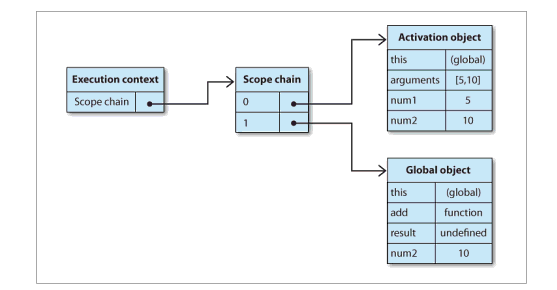
\includegraphics[width=1\textwidth]{figuras/scope_chain.png}
	\caption{Relación entre el contexto de ejecución y la \emph{scope chain}}
    \label{fig.scope_chain}
\end{figure}

Dentro de la función add, los identificadores \emph{num1} y \emph{num2} deben ser resueltos cuando la función esta ejecutando. Esta resolución se lleva a cabo inspeccionando
cada objeto en la \emph{scope chain} hasta que el identificador es encontrado. La búsqueda comienza con el primer elemento de la \emph{scope chain}, el cual es el registro
de activación que contiene las variables locales de la función. Si el identificador no es encontrado, el siguiente objeto de la \emph{scope chain} es inspeccionado en busca del
identificador.

Entender cómo funcionan los \emph{scopes} y las \emph{scope chain} en Javascript es importante, debido a que la performance de la resolución de identificadores esta directamente
relacionada al numero de objetos en la \emph{scope chain}.

\section{Variables locales}

Las variables locales son por lejos los identificadores más rápidos en los cuales se puede escribir y leer. Debido a que existen en los objetos de activación de la función
en ejecución, la resolución de identificadores involucra la inspección de un sólo objeto en la \emph{scope chain}. La cantidad de tiempo necesaria para leer el valor de una
variable aumenta con cada elemento que haya que inspeccionar en la \emph{scope chain}. Como las variables locales son las que se encuentran al comienzo de la \emph{scope chain}
son las mas rápidas de acceder, y por lo tanto es una buena práctica almacenar en variables locales todas las variables globales que sean referenciadas más de una vez
dentro de una función.

\section{La sentencia with}
La \emph{scope chain} para cierto contexto de ejecución normalmente no cambia durante la ejecución del código. Existen dos sentencias que temporalmente incrementan la
\emph{scope chain} de un contexto de ejecución. La primera es la sentencia with, que fue diseñada para permitir un acceso más simple a las propiedades de un objeto haciéndolas
parecer variables locales. Por ejemplo:

\begin{em}
var person = \{
    name: ``Nicholas'',
    age: 30
\};

function displayInfo()\{
    var count = 5;
    with(person)\{
        alert(name + `` is '' + age);
        alert(``Count is '' + count);
    \}
\}

displayInfo();
\end{em}

En esta función, el objeto \emph{person} es pasado en un bloque \emph{with}. Esto permite el acceso a las propiedades \emph{name} y \emph{age} como si hubieran sido definidas
de manera local. Lo que en verdad ocurre, es que un nuevo objeto es agregado al comienzo de la \emph{scope chain} del actual contexto de ejecucion.

\begin{figure}[h]
\centering
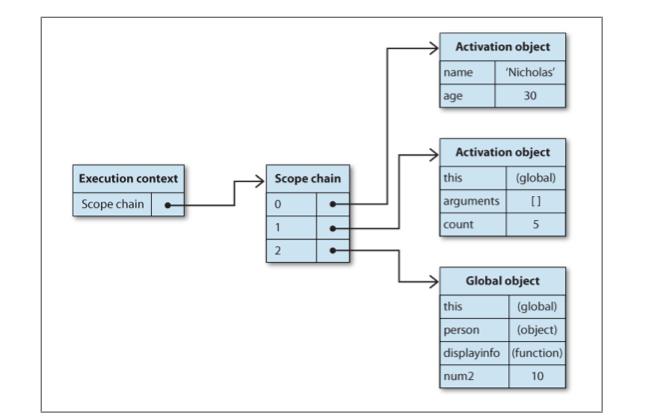
\includegraphics[width=1\textwidth]{figuras/scope_chain_with_statement.png}
	\caption{\emph{Scope chain} al utilizar la sentencia with}
    \label{fig.scope_chain_with_statement}
\end{figure}

Si bien el uso de esta sentencia puede parecer muy conveniente cuando las propiedades de un objeto son utilizadas con mucha frecuencia, este objeto extra en la
\emph{scope chain} del contexto daña la performance de la resolución de identificadores, debido a que las variables locales de la función pasan a encontrarse en el segundo
objeto en la \emph{scope chain}.

La sentencia \emph{catch} (correspondiente al bloque \emph{try catch}) es la segunda sentencia que aumenta el tamaño de la \emph{scope chain}. Ésta se comporta de manera
similar a la sentencia \emph{with} al agregar un objeto al comienzo de la \emph{scope chain} mientras ejecuta el código dentro del bloque. Ese objeto contiene una entrada
para la excepción especificada en la sentencia \emph{catch}. Sin embargo la sentencia \emph{catch} es ejecutada sólo cuando ocurre un error durante la ejecución de la
sentencia \emph{try}, resultando menos problemática que la snetencia \emph{with}.



\chapter{Selectores de CSS}
Entender como los navegadores parsean las reglas de estilo y renderizan las páginas web es una tarea importante al momento de mejorar la performance de una página web.
A medida que los navegadores parsean el documento HTML, construyen una estructura arborescente que representa todos los elementos que van a ser desplegados en la página.
Una vez completa esta etapa, busca las reglas que aplican a los elementos en diversas hojas de estilo, de acuerdo a las reglas de cascada, herencia y orden de CSS.

En la mayoría de las implementaciones de los navegadores, el motor de CSS busca reglas en las hojas de estilo que aplican a cada elemento del documento, evaluándolas de derecha a izquierda 
(debido a que el parser que utilizan es \emph{bottom-up}), empezando por el selector de más a la derecha, conocido como \emph{key} y
moviendose a través del selector hasta encontrar una concordancia o descartando la regla en otro caso.

En base a este sistema, mientras menos reglas tengan que ser evaludas por el motor de estilos, mejor será la performance del mismo. Por lo tanto remover reglas que no aplican es
un paso importante para mejorar la performance del renderizado, pero aún más importante es optimizar las definiciones de las reglas. Un aspecto clave al optimizar
las reglas de estilo, es definir reglas para que sean lo mas específicas posible y evitar redundancia en las mismas, para que de esta forma el motor de estilos pueda
encontrar rápidamente concordancias, evitando perder tiempo evaluando reglas que no aplican.

\section{Tipos de selectores}
En esta sección se listan los distintos tipos de selectores de CSS ordenados en base al costo en cuanto a la performance de los mismos, comenzando por los que tienen
menor impacto en la performance al momento de aplicar las reglas.

\subsection{Id}
Simple y eficiente, este selector aplica al único elemento en el documento HTML cuyo atributo \emph{ID} coincida con el de la regla.

\subsection{Clase}
Las reglas basadas en clases, se especifican con un punto seguido por el nombre de la clase. Los selectores de clase se aplican a todos los elementos que contengan la clase
de la regla en su atributo clase.

\subsection{Tipo}
Los selectores de tipo aplican a todos los elementos de un tipo especifico. La regla \emph{a\{text-decoration: none;\}} remueve el subrayado del texto de todos los
\emph{anchors} que se encuentren en la página. El uso de estas reglases una forma eficiente de agregar estilos a todos los elementos de un tipo especifico sin tener que
agregar caracteres extra, como clases a los elementos.

\subsection{Hermano adyacente}
Este selector consiste en concatenar dos selectores mediante el simbolo +. La regla \emph{h1 + \#toc} aplica al elemento que tiene \emph{toc} como atributo \emph{ID}, cuyo
hermano previo es un elemento del tipo \emph{h1}.

\subsection{Hijo \emph{child}}
Este tipo de selector es formado por la combinacion de dos o mas selectores simples mediante el uso del símbolo \emph{\textgreater}. La regla \emph{\#toc \textgreater   li \{font-weight: bold;\}}
aplica a todos los elementos del tipo \emph{li}, cuyo padre es el elemento con el atributo \emph{ID} igual a toc.

\subsection{Descendiente}
Estos selectores utilizan un espacio \emph{' '} como combinador. La siguiente regla \emph{\#toc a \{ color: \#444\}}, aplica a todos los elementos del tipo \emph{a} que sean
descendientes de el elemento cuyo \emph{ID} es igual a toc.

\subsection{Universales}
Los selectores universales (reglas representadas con un *) aplican a todos los elementos del documento.

\subsection{Atributo}
Los selectores por atributo aplican basandose en la existencia o valor de los atributos de un elemento. Un ejemplo de esto es la siguiente regla
\emph{[href='\#index'] \{font-style: italic;\}}.

\subsection{Pseudo-Clase y Pseudo-Elementos}
Este tipo de selectores son utilizados para aplicar a situaciones en las cuales la información no esta representada en el DOM. Algunas de las \emph{pseudo-classes} más
utilizadas son :hover, :visited, :first-child, :focus, etc.

\section{Reglas a evitar}

\subsection{No sobrecargar los selectores por Id}
Debido a que existe un único elemento en la página con un id específico, no es necesario agregar clasificadores extra ya que la única consecuencia que tiene esto es
retrasar el proceso. Por lo que es recomendable evitar reglas del estilo \emph{div\#toc}.

\subsection{No sobrecargar selectores de clase}
En vez de clasificar selectores de clase para etiquetas específicas, se recomienda extender el nombre de la clase para que sea específico con el caso de uso que se quiere
tratar. Por ejemplo, si se tiene una regla de este tipo \emph{li.chapter}, se recomienda cambiarla por \emph{.li-chapter} o mejor aun \emph{.list-chapter}.

\subsection{Reglas especificas}
La principal causa de la disminución de la eficiencia de la aplicación de los selectores es la existencia de múltiples etiquetas en una regla. Es mejor dividir estos
selectores en clases y agregarlas a los elementos correspondientes. Por ejemplo, es recomendable cambiar las reglas del tipo \emph{ol li a} por selectores de clases
del tipo \emph{.list-anchor}.

\subsection{Evitar selectores de descendencia y \emph{child}}
Los selectores por descendencia son los más costosos de procesar, debido a que por cada elemento que aplica a cada parte de la regla se debe evaluar otro nodo más. En
vez de estos es mejor utilizar clases asociadas a los elementos de la regla.

\subsection{Utilizar herencia de los atributos}
Muchas de las reglas de CSS se heredan, es mucho más costoso especificar este tipo de propiedades en cada elemento a tenerlas en un ancestro del mismo del cual
pueden heredarlas.


\chapter{JMeter}
JMeter es una una herramienta de escritorio desarrollada en Java y auspiciada por la Apache Software Foundation. Con este software libre, se pueden definir plantillas para programar baterías de test donde se simulen accesos concurrentes y medir de esta forma los tiempos de respuesta y el rendimiento global del sistema.

Esta herramienta puede ser utilizada como una herramienta de prueba de carga para analizar y medir el desempeño de una variedad de servicios, con énfasis en aplicaciones web.
JMeter puede ser usado como una herramienta de pruebas unitarias para conexiones de bases de datos con JDBC, FTP, LDAP, Servicios web, JMS, HTTP y conexiones TCP genéricas. 
JMeter puede utilizarse para evaluar la performance de recursos estáticos o dinámicos (archivos, servlets, objetos Java, bases de datos y queries, Servidores FTP, entre muchos otros). 

Se utiliza para simular una carga pesada sobre un servidor, red u objeto para analizar la performance total bajo diferentes tipos de carga. La herramienta puede utilizarse también para obtener análisis gráficos de la performance de la aplicación evaluada o testear el comportamiento de un servidor, script u objeto bajo grandes cargas concurrentes.
JMeter brinda muchas posibilidades y es por ello que es una de las herramientas más utilizadas en el mercado.

La herramienta permite realizar pruebas de carga y performance de diferentes tipos de servidores(Web, HTTP, HTTPS, SOAP. Database via JDBC, Mail-SMTP, POP3,IMAP). Además, es totalmente portable y está desarrollado en un 100\% en java. Además, brinda un framework para el manejo de múltiples hilos permitiendo una muestra concurrente mediante la ejecución de múltiples hilos y permitiendo una prueba simultanea por funcionalidad al definir diferentes grupos de hilos. Además, existen funciones para permitir el ingreso dinámico de datos a una prueba y la posibilidad de manipular dichos datos.
JMeter realiza muchas de las funcionalidades de un navegador al ejecutar una prueba, pero no todas. En particular, JMeter no ejecuta el Javascript que pueda encontrarse en las páginas HTML y tampoco renderiza dichos archivos HTML como lo haría un navegador.

\bibliographystyle{plain}
  \bibliography{apendice}

\end{document}
